\textit{Inverse dynamics} refers to the computation of the impulses given we
know the velocities of the system. It is shown in \cite{bib:todorov2014} that
this problem can be solved analytically given the separable structure of the
constraints. Then the impulse for each $k\text{-th}$ constraint can be solved
from
\begin{eqnarray}
	\bgamma_k&=&
	\begin{aligned}
		\argmin_{\bgamma\in\mathcal{C}} \quad &
	\frac{1}{2}(\bgamma-\mf{y}_k)^T\mf{R}_k(\bgamma-\mf{y}_k) \end{aligned}\\
	\mf{y}_k &=& -\vf{R}_k^{-1}(\mf{v}_{c,k}-\hat{\mf{v}}_{c,k})
\end{eqnarray}

From now on we will omit the index $k$. 

\subsection{Limits}
The solution for limits is trivial since $\mathcal{C}=\mathbb{R}^+$ or a finite
interval. \todo{summrize those results here.}

\subsection{Contact Impulses}

Contact impulses are constrained to the friction cone $\mathcal{C}=\mathcal{F}$.
This problem can be solved using simple geometry by noticing that the change of
variables $\tilde\bgamma=R^{1/2}\bgamma$ (and respectively
$\tilde{\vf{y}}=R^{1/2}\vf{y}$) leads to a projection with Euclidian norm on a
cone $\mathcal{F}_{\tilde\mu}$ with friction coefficient
$\tilde\mu=\mu\,(R_t/R_n)^{1/2}$
\begin{eqnarray}
	P_\mathcal{F_{\tilde\mu}}(\tilde{\vf{y}})&=&\argmin_{\tilde\bgamma\in\mathcal{F_{\tilde\mu}}}
		\quad \frac{1}{2}\Vert\tilde\bgamma-\tilde{\vf{y}}\Vert_2^2\nonumber\\
	P_\mathcal{F}(\vf{y}) &=&
	\vf{R}^{-1/2}P_\mathcal{F_{\tilde\mu}}(\tilde{\vf{y}})
	\label{eq:local_optimization_problem_tilde}
\end{eqnarray}

The optimization problem in the Euclidean norm given by Eq.
(\ref{eq:local_optimization_problem_tilde}) can be solved by inspection. If
$\tilde{\vf{y}}_i\in\tilde{\mathcal{F}}_i$, then we simply have
$\tilde{\bgamma}_i = \tilde{\vf{y}}_i$, we call this \textit{Region I}. If
however $\tilde{\vf{y}}_i$ is inside the negative of the dual cone (a.k.a. the
\textit{polar} cone), the closest point to $\tilde{\vf{y}}_i$ within the (tilde)
friction cone is zero, i.e. $\tilde{\bgamma}_i =\vf{0}$. We call this
\textit{Region III}. Finally, if $\tilde{\vf{y}}_i$ is in the region outside
both $\tilde{\mathcal{F}}_i$ and its polar $\tilde{\mathcal{F}}_i^\circ$, then
the closest point is it's Euclidian projection on the boundary of
$\tilde{\mathcal{F}}_i$. We call this \textit{Region II}. Figure
\ref{fig:cone_regions} shows a schematic of $\tilde{\mathcal{F}}_i$,
$\tilde{\mathcal{F}}_i^\circ$ and labels the three different regions. From Fig.
\ref{fig:cone_regions}, for a cone forming an angle $\theta$ with the z axis, we
have $\tan(\theta)=\tilde\mu$ and $\cos(\theta)=1/(1+\tilde\mu^2)$. Then the
projection can be written as
\begin{eqnarray}
	\tilde{\bgamma}_t &=& \tilde{\mu}\tilde{\gamma}_n\hat{\vf{t}}\nonumber\\
	\tilde{\gamma}_n &=& \frac{1}{1+\tilde{\mu}^2}\left(\tilde{y}_n +
	\tilde{\mu}\tilde{y}_r\right)\nonumber		
\end{eqnarray}
where $\tilde\mu=\mu(R_t/R_n)^{1/2}$ and the tangent vector is defined as
$\hat{\vf{t}}=\vf{y}_t/\Vert\vf{y}_t\Vert=-\vf{v}_t/\Vert\vf{v}_t\Vert$. 
\begin{figure}[!h]
    \centering
    %\vspace{6pt}
    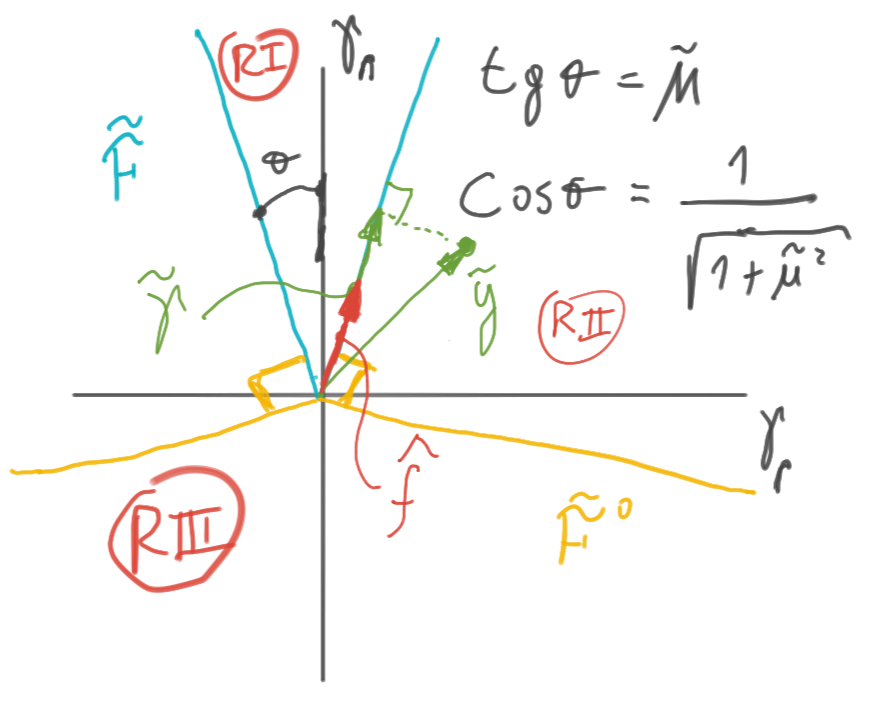
\includegraphics[width=0.45\columnwidth]{figures/cone_regions.png}
    \caption{Geometry of $\tilde{\mathcal{F}}_i$ and regions in the
    $\tilde{\vf{y}}$ space.}
    \label{fig:cone_regions}
\end{figure}

The desired expression for the original impulses
$\bgamma=\mf{R}^{-1/2}\tilde\bgamma$ in Region II is
\begin{eqnarray}
	\bgamma_t &=& \mu\gamma_n\hat{\vf{t}}\nonumber\\
	\gamma_n &=& \frac{1}{1+\tilde\mu^2}\left(y_n +
	\mu\frac{R_t}{R_n}y_r\right)\nonumber		
\end{eqnarray}

Finally, we can write the an analytical expression for $P_\mathcal{F}$ as
\begin{equation}
	\bgamma = P_\mathcal{F}(\vf{y}) = 
\begin{dcases}
	% Region I, stiction
	\vf{y} 
	% When we  have:
	& \text{stiction, } y_r < \mu y_n\\
	%
	%
	% Region II, sliding.
	\begin{bmatrix}
		\mu\gamma_n\hat{\vf{t}}\\
		\frac{1}{1+\tilde\mu^2}\left(y_n +
	\mu\frac{R_t}{R_n}y_r\right)
	\end{bmatrix}
	% When we  have:
	& \text{sliding, } -\mu \frac{R_t}{R_n} y_r < y_n \leq \frac{y_r}{\mu}\\
	%
	%
	% Region III, no contact.
    \vf{0} & \text{no contact, } y_n \leq -\mu \frac{R_t}{R_n} y_r
\end{dcases}	  
	\label{eq:inverse_dynamics_projection}
\end{equation}
where $\vf{y}_t$ and $y_n$ are the tangential and normal components of $\vf{y}$,
the radial component is defined as $y_r=\Vert\vf{y}_t\Vert$ and the tangent
vector as $\hat{\vf{t}}=\vf{y}_t/y_r$. We also defined the common dimensionless
factors $\tilde\mu=\mu\,(R_t/R_n)^{1/2}$ and $\hat\mu=\mu\,R_t/R_n$.
